\chapter{\label{ch:3-orion}Attosecond X-ray harmonics on the ORION laser facility} 

\minitoc

\section{A plan}
This chapter reports on the March 2023 experiment at the ORION laser facility, AWE, Aldermaston. The UK's most powerful sub-picosecond laser.

Important sections include:
HYADES scale length sims, ORION parameters and description of the setup, targets etc, data analysis after, beamlet sims, HHG theory


I think the appropriate order would be theory, simulation, experiment layout, data analysis since then I can use all things inferred from theory and simulation to justify the data analysis. It also means ending well.


\section{\label{ch:3-sec:theory}Theory}

\subsubsection{Hole boring}
% TODO add reference to ZVP plots demonstrating hole boring.
As observed in the ZVP plots, on long timescales relative to the laser pulse cycles, via the ponderomotive pressure of the laser, the plasma front moves inwards. This is hole boring \cite{wilksAbsorptionUltraIntenseLaser1992}. One can derive a hole boring velocity by considering conservation of momentum in this quasi-static state. Since the hole boring velocity is laser pulse intensity dependent, the spatial profile of the laser will be imprinted on the surface. Typically Gaussian in shape, for high power laser systems, this can to first order generate a focusing \ac{RPM} and a beaming of the specularly reflected signal, as in Figure \ref{fig:orionholeboring}.
\begin{figure}
	\centering
	\includegraphics[width=0.7\linewidth]{figures/orion/orion_hole_boring}
	\caption[2D PIC simulation of HHG beaming effect via hole boring.]{Electromagnetic field intensity in a 2D PIC simulation of a relativistic ($a_0 = 30$) laser pulse incident on a solid density plasma. The incoming beam is specularly reflected off the target which is curved by the radiation pressure leading to beaming in the reflected harmonic beam.}
	\label{fig:orionholeboring}
\end{figure}
To access the highest possible electromagnetic field intensities, the laser pulse is focused on target to the diffraction limit. However, since the diffraction limit scales linearly with the wavelength, higher-order harmonics can be refocused to a smaller spot via this mechanism allowing access to unprecedented peak intensities. Vincenti \textit{et al} demonstrated intensity gains of over 1000 with currently accessible parameters in \ac{3D} \ac{PIC} simulations \cite{vincentiAchievingExtremeLight2019}, suggesting a realistic route to the Schwinger Limit using next-generation laser facilities. Regardless of any blue-skies purposes, it is clear any prediction of \ac{HHG} beam intensity must account for hole boring and is therefore an essential component of the ORION experiment analysis.

% TODO I might want to flesh out the hole boring analysis but it already takes up so much space so idk...
Applying momentum balance between the laser pulse and particles in the rest frame of the \ac{RPM} surface, the hole boring velocity is
\begin{equation}\label{eq:v_HB}
	\frac{v_\mathrm{HB}}{c} = \sqrt{\frac{R\cos\theta}{2}\frac{Zm_\mathrm{e}}{Am_\mathrm{p}}\frac{n_\mathrm{c}}{n_\mathrm{e}(x_\mathrm{i}(t,y))}}a_L(t,y) = \Pi a_L(t,y),
\end{equation}
where $R$ is the RPM reflectivity, $\theta$ is the angle of incidence, \qty{16}{\degree} in the ORION experiment, $Z$ and $A$ are the atomic and atomic mass numbers respectively for the plasma ions, $n_\mathrm{c}$ is the plasma critical density, $n_\mathrm{e}(x_\mathrm{i}(t,y))$ the electron number density and $x_\mathrm{i}(t,y)$
the depth of hole boring, from the Supplementary Material \cite{vincentiOpticalPropertiesRelativistic2014}. For the ORION laser pulse parameter space $\Pi \ll a_\mathrm{L}$, hence the relativistic correction derived by Robinson \textit{et al} \cite{robinsonRelativisticallyCorrectHoleboring2009} to Equation \ref{eq:v_HB} can be neglected. Due to the high contrast and long duration of the ORION beamlines, there is effectively no pre-plasma formation on the front surface and therefore the number density is simply the number density of the material in solid form and $n_\mathrm{e}$ is independent of $x_\mathrm{i}(t,y)$. Robinson \textit{et al} \cite{robinsonHoleboringRadiationPressure2009} calculated a generalisation of momentum conservation to multiple species, simply replace the mass density with the composite mass density $\rho = \sum_j m_{\mathrm{i}j}n_{\mathrm{i}j}$, then
\begin{equation}
	\frac{An_\mathrm{e}}{Z} \to \sum_j \frac{A_jn_{\mathrm{e}j}}{Z_j},
\end{equation}
where $n_{\mathrm{e}j}$ is the number density of electrons that originated from the $j$ ion.


%TODO (This analysis can be done by taking the Vincenti 2014 derivation and taking $R =1$, since that applied to ORION parameter space, replace ion terms with sums over ions and make the important assumption: all ions reflected at the same velocity (reasonable), note that this might be a tricky to do to electrons when there is significant electron heating and so $R < 1$, may need to return to this for thesis... manipulating the expression arrives at the desired form)

The spatio-temporal envelope of the normalised vector potential of the laser pulse incident on the target surface is modelled as
\begin{equation}
	a_\mathrm{L}(t,y) = a_0e^{-\frac{y^2}{2w_\mathrm{L}^2}}g(t-t_0)
\end{equation}
where $w_\mathrm{L}$ is the beam waist on target and $g(t)$ the temporal envelope, a Gaussian or $\sech$ profile and $t_0$ the main pulse peak time.

Integrating equation \ref{eq:v_HB},
\begin{equation}\label{eq:xi_t}
	x_\mathrm{i}(y) = \int v_\mathrm{HB}\mathrm{d}t = \Pi \int^t_{-\infty} a_L(t,y)c\mathrm{d}t.
\end{equation}

At the peak of the main pulse,
\begin{equation}
	x_\mathrm{i}(y) = \Pi a_0ce^{-\frac{y^2}{w_L^2}} G,
\end{equation}
where $G = \int_\infty^{t_0} g(t-t_0) \mathrm{d} t \sim t_\mathrm{p}$, where $t_\mathrm{p}$ is the pulse duration.

The total denting is a combination of the peak electron-ion charge separation, $x_\mathrm{e}$ (which leads to the intrinsic phase imprint on the HHG beam) and equation \ref{eq:xi_t}. Note that for the long pulse duration of the ORION laser, $x_\mathrm{i} \gg x_\mathrm{e}$ and therefore $x_\mathrm{e}$ can be neglected.

Applying a Taylor expansion to the spatial profile of equation \ref{eq:xi_t} around the laser spot centre,
\begin{equation}
	x_\mathrm{i} = \mathrm{constant} - \frac{y^2}{4f_\mathrm{p}} + \mathcal{O}(y^4),
\end{equation}
where, to first order, this is the equation of a parabolic mirror with focal length
\begin{equation}
	f_\mathrm{p}(t) = \frac{w_\mathrm{L}^2}{4\Pi\int^t_{-\infty} a_0\exp({-t^2/2t^2_\mathrm{p}})c\mathrm{d}t}.
\end{equation}

Following the Vincenti \textit{et al} derivation \cite{vincentiOpticalPropertiesRelativistic2014}, the denting parameter is defined as,
\begin{equation}
	\delta_\mathrm{T} =  x_\mathrm{i}|_{(y=0)} - x_\mathrm{i}|_{(y=\sqrt{2}\omega_\mathrm{L})}.
\end{equation}
Hence,
\begin{equation}
	\delta_\mathrm{T} = \frac{w_\mathrm{L}^2}{2f_\mathrm{p}} = 2\Pi \int^t_{-\infty} a_0 e^{-t^2/2t^2_\mathrm{p}}c\mathrm{d}t,
\end{equation}
and is independent of laser focal spot size. 

If the spatial profile of the $n^\mathrm{th}$ harmonic beam can be adequately described by a Gaussian at the plasma mirror plane, with a beam width described by the harmonic source size, $w_n$,
\begin{equation}
	h_n \sim e^{-r^2/w_n^2},
\end{equation}
then the beam profile is known at all distances, $z$ from the target. Its divergence, defined as 
\begin{equation}
	\theta_n = \lim_{z\to\infty} \frac{w_n(z)}{z},
\end{equation}
is therefore
\begin{equation}
	\theta_n = \theta^0_n\sqrt{1+\Psi^2_n},
\end{equation}
where $\theta^0_n = \lambda_n/\pi w_n$ is the harmonic divergence in the absence of RPM denting and
\begin{equation}
	\Psi_n = \frac{2\pi}{\cos\theta}\left(\frac{w_n(0)}{w_L}\right)^2\frac{\delta_T}{\lambda_n}
\end{equation}
is the dimensionless focusing parameter. If $\Psi_n \gg 1$, as is true for the short wavelength X-ray harmonics of interest, 
\begin{equation}
	\theta_n \approx \frac{w_n(0)}{f_\mathrm{p}\cos\theta}
\end{equation}
and the divergence is dominated by RPM curvature. 

Far from focus, at the detector plane $z =$ 2.4 m from the target,
\begin{equation}
	w_{n} \approx z\tan\theta_n.
\end{equation}
The corresponding magnification factor at detection is thus 
\begin{equation}
	\gamma_n(z) = \frac{w_n(z)}{w_n(0)},
\end{equation}
thus the laser intensity at detection is reduced by a factor $\gamma_n(z)^{-2}$.

Note that at large distances,
\begin{equation}
	\gamma_n \approx \frac{z\tan(w_n(0)/(f_\mathrm{p}\cos\theta}{w_n(0))},
\end{equation}
Taylor expanding the tangent, one sees that the magnification factor is only weakly dependent on the harmonic source size ($f_\mathrm{p}$ is independent of the source size), whereas the magnification is strongly dependent on the the laser spot size ($\sim w_\mathrm{L}^4$).


At the new focal point, $z = z_\mathrm{f}$, the demagnification factor is \cite{vincentiOpticalPropertiesRelativistic2014}
\begin{equation}
	\gamma_n(z_\mathrm{f}) = \frac{1}{\sqrt{1+\Psi_n^2}},
\end{equation}
this determines the new peak intensity accessible using this technique.


%TODO mention intrinsic phase and explain neglections.

\section{\label{ch:3-sec:data_processing}Experimental data processing}

\subsection{Image plate calibration}
Image plates (IPs) are reusable recording media that detect ionising radiation and are particularly suitable for the detection of X-rays produced in laser-plasma interactions. Their response is well understood and their sensitivities to a wide spectrum photon energies have been absolutely calibrated on the ORION facility \cite{meadowcroftEvaluationSensitivityFading2008}. Albeit for the FLA3000 scanner not the FLA7000 used in this experiment. However, the deviation in response is negligible for the photon energies measured. In this experiment the Fuji Biological Analysis System (BAS) TR-type IPs were used. They have a phosphor layer composed of $\mathrm{BaFBr_{0.085}I_{0.15}}$ with density \qty{2.61}{g.cm^{-3}} and thickness \qty{60}{\mu m} but no mylar layer. This makes them suitable for low energy X-ray detection. When scanned, the IP releases blue photons via photostimuated luminescence (PSL), which is then collected by a photomultiplier tube. The PSL value is generalised across scanner types from the measured `Grey' ($G$) value by
\begin{equation}
	\mathrm{PSL} = (0.23284G^2\times 10^{-9})\left(\frac{\Delta x}{100}\right)^2W\times 10^{-L/2},
\end{equation}
where $\Delta x$ is the scanner resolution (= \qty{25}{\mu m} in this experiment), $L$ is the latitude parameter, and
\begin{equation}
	W = 0.092906 + 1370.8e^{-0.014874V} +  654.24e^{-0.011026},
\end{equation}
where $V$ is the scanner voltage \cite{golovinCalibrationImagingPlates2021}.

IP photon sensitivity, $\psi$, the number of PSLs per incident photon, is dependent on photon energy. Meadowcroft \textit{et al} modelled this as,
\begin{equation}
	\psi_j = \eta(m_jh\nu + c_j),
\end{equation}
where $h\nu$ is the photon energy and $m_j$ and $c_j$ are linear fit parameters valid for specific energy ranges, $j$. For the Fuji BAS TR-type IP and for X-rays in the range 0-6.0 keV, $m_j = \qty{0.54\pm0.05}{mPSL.keV^{-1}}$ and $c_j = \qty{0.02\pm0.002}{mPSL}$. The IP absorption efficiency in mPSL per photon is
\begin{equation}
	\eta(h\nu,T_i,T_s) = \exp{(-n_\mathrm{i}\Phi_\mathrm{i} (h\nu)T_\mathrm{i})}[1-\exp{(-n_\mathrm{s}\Phi_\mathrm{s}(h\nu)T_\mathrm{s})}],
\end{equation}
where $n$ is the layer density, $\Phi(h\nu)$ is the total cross-section of the layer, $T$ the effective layer thickness, s and i correspond to the sensitive (phosphor) and insensitive (mylar) layers of the IP respectively \cite{izumiApplicationImagingPlates2006}. The first term is neglected in the absence of an insensitive (mylar) layer in TR-type IP. Below 50 keV, the dominant mode for X-ray absorption into the IP is the photo-electric effect, where
\begin{equation}
	\Phi_\mathrm{ph} \approx \num{3e12}\frac{Z^4}{(h\nu)^{3.5}}   
\end{equation}
and $Z$ is the atomic number \cite{fornalskiSimpleEmpiricalCorrection2018} and $\Phi_\mathrm{ph}$ is given in units of Barn per atom. At 2.4 keV, that corresponds to a sensitivity of 1.32 mPSL per incident photon.

It is generally inevitable that some time will elapse between laser shot and IP scan. For this experiment 30 minutes was typical, in which time some fading of the IP occurs that must be accounted for. IP fading can be modelled as an attenuation factor,
\begin{equation}\label{eq:orion.Ft}
	F(t) = A\exp{(-t/\tau)} + B,
\end{equation}
where $t$ is the time between shot and scan and $A$, $\tau$ and $B$ are found from fits to experimental data. A key aspect of the exponential decay is that the attenuation depends only on the signal at that moment in time and not the initial conditions. This has been shown to be true in experiment \cite{meadowcroftEvaluationSensitivityFading2008}.

At \qty{20}{\degree C} at the ORION facility \textit{Meadowcroft et al} \cite{meadowcroftEvaluationSensitivityFading2008} determined that for the Fuji BAS TR-type IP, the optimum fit for the parameters of equation \ref{eq:orion.Ft} is $A = \num{0.347\pm0.022}$, $B = \num{0.693\pm0.011}$ and $\tau = \qty{35.5\pm5.3}{minutes}$. Therefore at 30 minutes, $F(t) = 0.84$.

In summary, the number of PSL measured on an IP can be converted to an incident number of photons via
\begin{equation}
	N(h\nu) = \frac{\mathrm{PSL}}{F(t)}\frac{10^3}{\psi(h\nu)} = P(h\nu) \mathrm{PSL}.
\end{equation}

\subsection{OHREX calibration}
% TODO Reword note on illuminating crystal once I have written up about hole boring.
The Orion High REsolution X-ray spectrometer (OHREX), housed on the ORION laser target chamber outer wall, utilises a spherically bent crystal geometry to spatially focus and spectrally analyse photons from the target chamber \cite{beiersdorferLineshapeSpectroscopyVery2016} with a high signal-to-noise ratio. The measured signal has been absolutely calibrated for a range of energies using a variety of crystals \cite{macdonaldAbsoluteThroughputCalibration2021}. The OHREX can hold two crystals at a time. At each crystal's spatial focal plane a two-dimensional image is formed, one dimension is spatial, the other spectral. The energy range accessed by a given crystal is determined by the crystal rotation but all OHREX crystals are designed for operation at a nominal central Bragg angle of $\theta_\mathrm{B} = 51.3$\degree with the corresponding wavelength determined from Bragg's Law, $n\lambda = 2d\sin\theta_\mathrm{B}$, for the appropriate crystal plane. The range around that central photon energy is determined by the crystal width in the spectral dimension.

MacDonald \textit{et al} determined a quadratic fit for each crystal's dispersion relation to connect position along the image to photon energy \cite{macdonaldAbsoluteThroughputCalibration2021}. Unfortunately in this experiment, the image lengths varied from those in the previous experiment, a likely consequence of slight defocusing of the optic. Note that the OHREX geometry is designed such that precise focus is not necessary to achieve good results \cite{beiersdorferLineshapeSpectroscopyVery2016}.

Instead, a simple linear dispersion relation based on the known maximum and minimum energies accessed by the crystal was applied across the crystal images, a reasonable approximation to the dispersion relation determined by MacDonald \textit{et al} \cite{macdonaldAbsoluteThroughputCalibration2021} (the quadratic correction is small). The energy ranges for the three lowest energy OHREX crystals are given in table \ref{tab:dispersion}.
\begin{table}
	\centering
\begin{tabular}{ccc}
	\hline \hline
	Crystal               & Range, $n=1$ (eV) & Range, $n=2$ (eV) \\ \hline
	KAP (100)             & 585-625          & 1170-1245        \\
	Quartz ($10\bar{1}0$) & 1830-1950        & 3660-3900        \\
	Quartz ($10\bar{1}1$) & 2330-2480        & 4660-4960  \\     \hline \hline
\end{tabular}
	\caption{\label{tab:dispersion} Photon energy ranges captured by the three lowest energy OHREX crystals when operating at their nominal central Bragg angle of 51.3\degree for first and second diffraction orders, $n$.}
\end{table}

Provided full illumination of the \qty{6}{cm} $\times$ \qty{4}{cm} crystal, the spatial dimension can be safely integrated over to calculate the measured signal, $M(h\nu)$ in \unit{J.mm^{-1}} and remove uncertainty from the IP drifting from the ideal focal plane. (In this experiment we assume that the harmonic beam width at the crystal position is larger than the size of the crystal, a reasonable assumption since beam divergence $\approx$ \qty{10}{\degree} and the \qty{6}{cm} x \qty{4}{cm} crystal sits \qty{2.4}{m} from the target.). This corresponds to a source spetral intensity incident on the crystal $S(h\nu)$ measured in \unit{J.keV^{-1}.sr^{-1}} via the spectrometer response, $G(h\nu)$, explicitly,
\begin{equation}
	M(h\nu) = S(h\nu)G(h\nu).
\end{equation}
The absolute throughput of the crystals was measured by MacDonald \textit{et al} in a previous ORION experiment and fit parameters for 
\begin{equation}
	G(h\nu) = A(h\nu)^2 + B(h\nu) + C,
\end{equation}
where $(h\nu)$ is the photon energy measured in eV, determined for both p- and s-polarised incident light and for first and second diffraction orders \cite{macdonaldAbsoluteThroughputCalibration2021}. The parameters for the lowest few energy crystals are presents in Table \ref{tab:orion_OHREX}.
\begin{table}
\centering
\begin{tabular}{cccccc}
	\hline \hline
	Crystal               & Order & Polarisation & $A$            & $B$             & $C$            \\
	\hline
	KAP             & 1     & s            & \num{1.72e-15} & \num{-4.69e-12} & \num{2.89e-9}  \\
	(100) &       & p            & \num{1.40e-14} & \num{-1.74e-11} & \num{5.42e-9}  \\
	& 2     & s            & \num{3.64e-16} & \num{-9.64e-13} & \num{6.95e-10} \\
	&       & p            & \num{5.03e-10} & \num{8.09e-13}  & \num{5.03e-10} \\
	Quartz  & 1     & s            & $\cdots$       & $\cdots$        & $\cdots$       \\
	  ($10\bar{1}0$)&     & p            & $\cdots$       & $\cdots$        & $\cdots$       \\
	& 2     & s            & \num{4.50e-15} & \num{-3.40e-11} & \num{6.52e-8}  \\
	&       & p            & \num{1.13e-15} & \num{-8.86e-12} & \num{1.73e-8}  \\
	Quartz  & 1     & s            & \num{1.00e-16} & \num{-1.74e-12} & \num{4.93e-9}  \\
	  ($10\bar{1}1$)&     & p            & \num{2.78e-15} & \num{-1.41e-11} & \num{1.79e-8}  \\
	& 2     & s            & \num{4.70e-16} & \num{-4.50e-12} & \num{1.11e-8}  \\
	&       & p            & \num{2.10e-16} & \num{2.11e-12}  & \num{5.30e-9}  \\
	\hline \hline
\end{tabular}
\caption{Sensitivity fit parameters as a function of photon energy, $h\nu$ in electron-volts ($G(h\nu) = A(h\nu)^2 + B(h\nu) + C$) for the three lowest energy OHREX crystals for p- and s-polarised incident photons and first and second diffraction orders \cite{macdonaldAbsoluteThroughputCalibration2021}. Note that no data is available for the first order of the quartz ($10\bar{1}0$) crystal.}
\label{tab:orion_OHREX}
\end{table}
There is unfortunately no spectrometer response data for the $10\bar{1}0$ crystal to first order due to the Si K edge sitting within the energy range and the dramatic effect this has on absorption in its vicinity \cite{hellCalibrationOHREXHighresolution2016}.


The OHREX is equipped with a \qty{50}{\mu m} Beryllium filter to protect the crystals. The corresponding signal attenuation can be calculated using X-ray transmission data \cite{henkeXRayInteractionsPhotoabsorption1993a}.

\subsection{Extracting the data}
The quartz OHREX crystals $10\bar{1}0$ and $10\bar{1}1$ were fielded on the experiment. Crystal images were recorded with BasTR2040 Fuji Image Plate. A typical shot image scanned with the FLA7000 scanner and converted to photostimulated luminescence units (PSLs) is given in figure \ref{fig:orionohrexshot28psl}.
%todo point out both crystal images and label them
\begin{figure}
	\centering
	\includegraphics[width=0.5\linewidth]{figures/orion/orion_OHREX_shot28_psl}
	\caption[Unprocessed IP from ORION experiment]{Unprocessed shot data from a FLA7000 scanned image plate converted to PSLs. The image plate and two crystal images are clearly visible.}
	\label{fig:orionohrexshot28psl}
\end{figure}
The average background signal was subtracted. The $x$- and $y$-axes were converted from pixels to to mm using the scanner resolution, (\qty{25}{\mu m.px^{-1}}) and then energies using the appropriate dispersion relations. The data was then integrated over $y$ to obtain the intensity in units of \unit{PSL.mm^{-1}} across each crystal image. Then the corresponding source signal is
\begin{equation}
	S(h\nu)[\unit{J.keV^{-1}.sr^{-1}}] = \frac{d\mathrm{PSL}}{dx}\frac{P(h\nu)}{G(h\nu)}h\nu,
\end{equation}
which can then be converted to a measured spectral intensity per harmonic at distance $r=1$ from the source, ready to be directly compared to the theory,
\begin{equation}
	I^\mathrm{meas}_\mathrm{n}|_{(r = \qty{1}{m})} = S(h\nu)\frac{dh\nu(keV)}{dn}.
\end{equation}

No sensitivity data is available for the $10\bar{1}0$ quartz crystal, instead this lower energy crystal was fielded to attempt resolving of the X-ray harmonics. At the experiment planning stage it was unknown if this would be possible. Now that the simulations have been performed, we know that the non-optimal ORION target chamber geometry leads to merging of the harmonics even before the water window at 282 eV. This is consistent with the findings, Figure \ref{fig:orionq1010} is a typical integrated signal in \unit{PSL.mm} and the corresponding Fourier transform for the quartz ($10\bar{1}0$) crystal image.
\begin{figure}
	\centering
	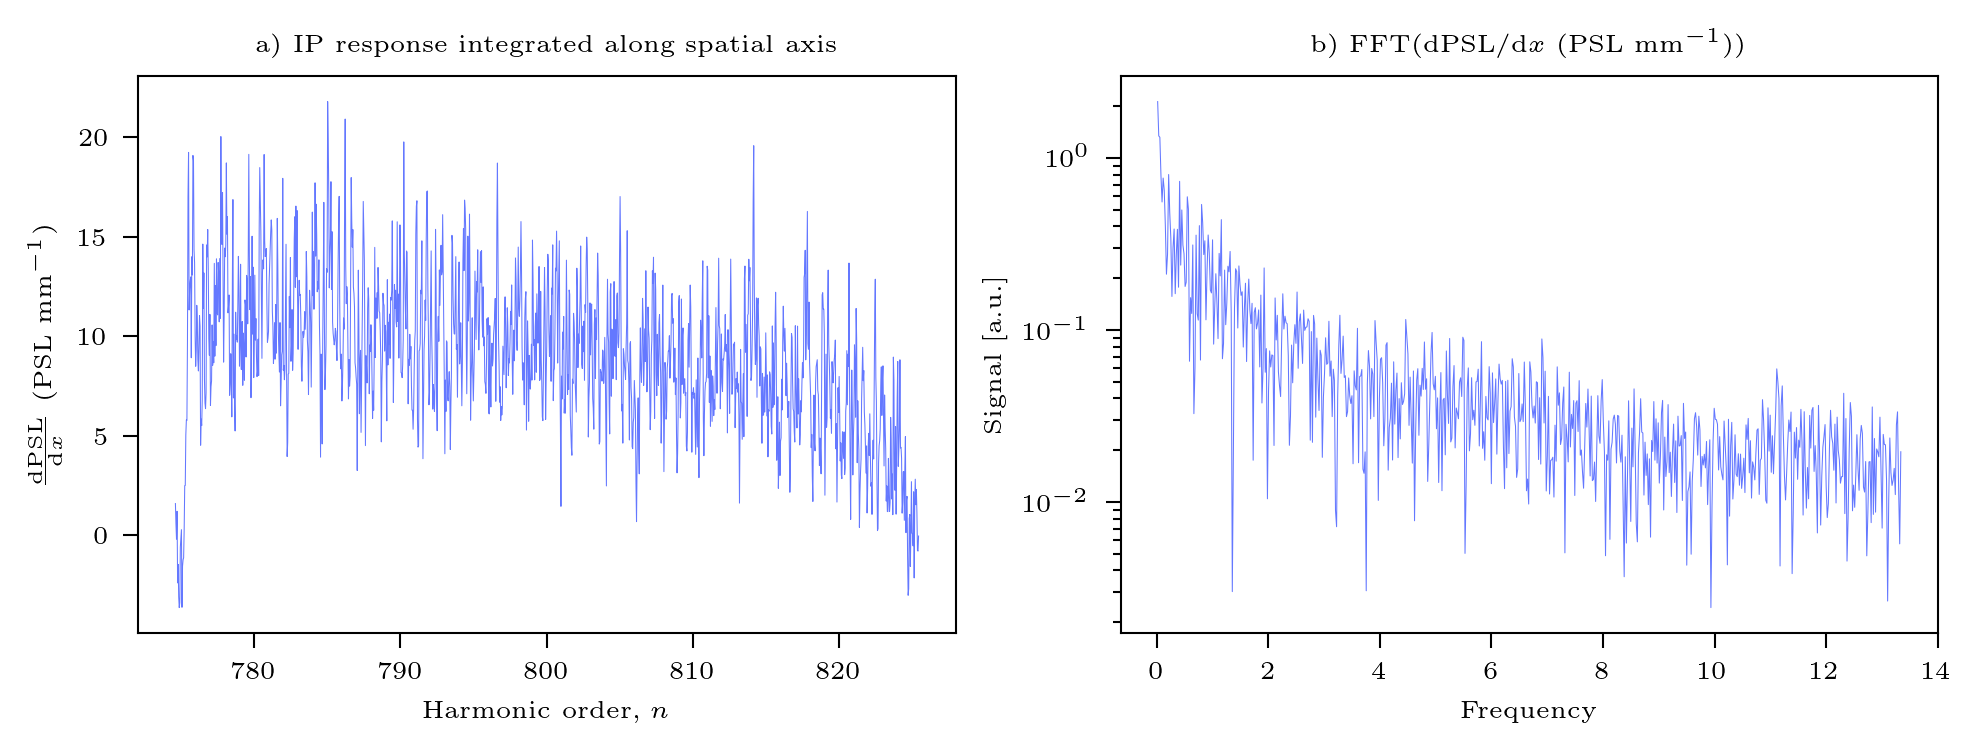
\includegraphics[width=1\linewidth]{figures/orion/orion_q1010}
	\caption[Typical ORION experiment uncalibrated IP response quartz ($10\bar{1}0$) crystal and Fourier transform]{\textbf{Typical (SP1, PMMA) uncalibrated shot data for the quartz ($10\bar{1}0$) image} a) IP spatial axis integrated signal with dispersion axis. b) Fourier transform of a) with no evidence of harmonics.}
	\label{fig:orionq1010}
\end{figure}

\subsubsection{Calibration and polarisation}
% TODO reference simulation figure that shows only p pol light reflected.
% TODO write up the OHREX polarisation stuff
% TODO put efficiency of only p pol reflected into the theory prediction, I think at this moment I am coming at it from the experiment side which is wrong.
% TODO add in polarisations of SP1 and SP2 for the OHREX angles out of the plane.
The choice of the spectrometer response function, $G(h\nu)$, is non-trivial. One must firstly be assured that the second order contribution is small relative to the first, true for this source spectrum. And also think carefully about the anticipated polarisation in the OHREX interaction plane. The OHREX response to p-polarised light is approximately an order of magnitude lower than for s-polarised light. From Figure X we are assured that only the p-polarised (with respect to the target interaction plane) X-rays are specularly reflected to the OHREX. Corresponding polarisation out of the OHREX interaction plane is calculated in the Appendix. The polarisation of the HHG beam relative to the OHREX plane of incidence and reflection is \qty{10.5}{\degree} out of the plane. Unlike for the RPM interaction, the OHREX crystal reflection is an entirely linear process and it is therefore acceptable to decompose the laser pulse into its constituents, explicitly, the field incident on the crystal is
\begin{equation}
	\mathbf{E_\mathrm{O}} = \mathbf{E}_\mathrm{O,\, s} + \mathbf{E}_\mathrm{O,\, p}.
\end{equation}
After interaction with the crystal the field is
\begin{equation}
	\mathbf{E}_\mathrm{detector} = \alpha_\mathrm{s}(h\nu)\mathbf{E}_\mathrm{O,\, s} + \alpha_\mathrm{p}(h\nu)\mathbf{E}_\mathrm{O,\, p},
\end{equation}
where $\alpha_i(h\nu)$ is the energy dependent $(h\nu)$ amplitude sensitivity of the reflection for s- and p-polarised respectively. Since the two polarisations are orthogonal, the intensity is
\begin{equation}
	I = \alpha^2_\mathrm{s}(h\nu)|\mathbf{E}_\mathrm{O,\, s}|^2 + \alpha^2_\mathrm{p}(h\nu)|\mathbf{E}_\mathrm{O,\, p}|^2.
\end{equation}
Noting that $\alpha^2_i(h\nu)$ are the calibration factors, $G_i(h\nu)$, and that
\begin{equation}
	|\mathbf{E}_\mathrm{O,\, s}| = |\mathbf{E_\mathrm{O}}|\sin\phi
\end{equation}
and
\begin{equation}
	|\mathbf{E}_\mathrm{O,\, p}| = |\mathbf{E_\mathrm{O}}|\cos\phi,
\end{equation}
where $\phi$ is the angle out of the interaction plane,
\begin{equation}
	I_\mathrm{detector} = (G_\mathrm{s}(h\nu)\sin^2\phi + G_\mathrm{p}(h\nu)\cos^2\phi)|\mathbf{E_\mathrm{O}}|^2 = F(h\nu)|\mathbf{E_\mathrm{O}}|^2,
\end{equation}
where $F(h\nu) =  (G_\mathrm{s}(h\nu)\sin^2\phi + G_\mathrm{p}(h\nu)\cos^2\phi$ is the energy dependent calibration factor for this OHREX orientation.


Figure \ref{fig:orionq1011} is a typical calibrated signal from the quartz ($10\bar{1}1$) crystal, ready for comparison to the theoretical prediction.
\begin{figure}
	\centering
	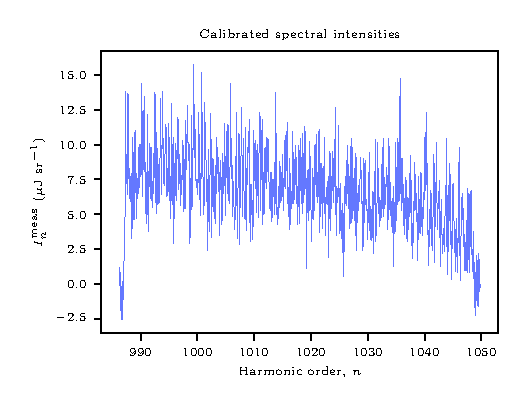
\includegraphics[width=0.7\linewidth]{figures/orion/orion_q1011}
	\caption[Typical ORION experiment calibrated IP response for the quartz ($10\bar{1}1$) crystal.]{Typical (SP1, PMMA) ORION experiment calibrated IP response for the quartz ($10\bar{1}1$) crystal.}
	\label{fig:orionq1011}
\end{figure}



Shots were also taken through the OHREX port, we had hoped to capture the beam divergence however, the beam was larger than initially expected and we were unable to distinguish much. Mention saturation.


Once done all this analysis, present the data.. Integrated signal across crystal, discuss no harmonics but that is expected and then present the final table and discuss. 

Include a table detailing error contributions? Also need to add reflectivity error to the rest.

Discuss mirrored targets and brems emission.

Then go back and do the theory. then sims.

Also in sims look at reconstructing a filtered pulse
